\documentclass[defaultpackages]{cheatsheet}

\usepackage{lipsum}

\usepackage{graphicx}

\title{An example cheatsheet}
\author{Teodor Dahl Knutsen}

\begin{document}

\tableofcontents

\section{Det første som skjer}

\lipsum[1-1]

\begin{equation}
	\sum_{n=1}^\infty 10^{-n!}=0.110001\cdots\label{eq_1}
\end{equation}

As you can see in Equation~\ref{eq_1}, it is a transcendental number, $3 + 5 = 8$.

\lipsum[2-2]

\[ \int_0^\infty f(x)\, dx = e^x \]

\lipsum[1-1]

\subsection{Enda en test}

\begin{figure}[H]
\begin{center}
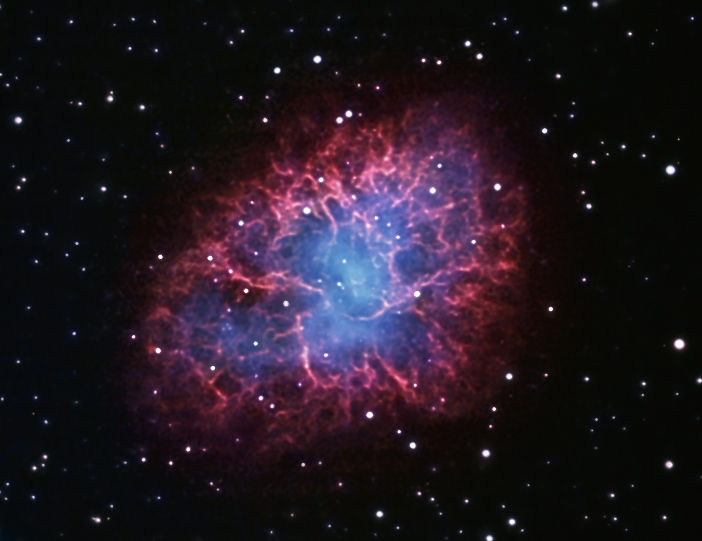
\includegraphics[width=50px] {crab_nebula.jpg}
\end{center}
\caption{A binary search tree, but this caption is a lot longer. Trying to make it a lot of lines to test spacing in the captions.}\label{fig:ackseq}
\end{figure}

\lipsum[1-1]

\section*{Unnumbered section}

\subsubsection{Lorem ipsum dolor sit amet}

\lipsum[1-1]

\section{kake}

\lipsum[3-50]

\end{document}
